% %
% LAYOUT_E.TEX - Short description of REFMAN.CLS
%                                       99-03-20
%
%  Updated for REFMAN.CLS (LaTeX2e)
%
\documentclass[twoside,a4paper]{refart}
\usepackage{makeidx}
\usepackage{ifthen}
\usepackage{url}
\usepackage{csquotes}
\usepackage{graphicx}
\usepackage{float}
\usepackage{caption}
\usepackage{hyperref}



% ifthen wird vom Bild von N.Beebe gebraucht!

\def\bs{\char'134 } % backslash in \tt font.
\newcommand{\ie}{i.\,e.,}
\newcommand{\eg}{e.\,g..}
\DeclareRobustCommand\cs[1]{\texttt{\char`\\#1}}
\captionsetup{hypcap=false}

\title{\LaTeX\ Guide Guide}
\author{
John Pan (jpthek9@gmail.com)\\
\url{https://github.com/SnpM}
}

\date{\url{https://github.com/SnpM/latex-guide-guide.git}\\\today}
\emergencystretch1em  %

\pagestyle{myfootings}
\markboth{\LaTeX\ Guide Guide}%
         {\LaTeX\ Guide Guide}

\makeindex 

\setcounter{tocdepth}{2}

\begin{document}

\maketitle

\begin{abstract}
         \LaTeX\ is a typesetting standard for academic and professional documents. The system may seem complicated because of its coding syntax, but powerful \LaTeX\ editors such as Overleaf streamline the learning the process. A wealth of high-quality \LaTeX\ templates exist online, enabling authors to focus on content rather than appearance. This guide describes how to author an instructional \LaTeX\ document in Overleaf using the \texttt{refman} template.
\end{abstract}

This document is part of my final project for the Technical Communication course at Thomas Edison State University, mentored by Dr. Douglas Hoehn. 

\tableofcontents

\newpage


%%%%%%%%%%%%%%%%%%%%%%%%%%%%%%%%%%%%%%%%%%%%%%%%%%%%%%%%%%%%%%%%%%%%

\section{Introduction}

%Cut Subsections%


{\subsection{What is \LaTeX?}
LaTeX (pronounced \enquote{Lay-Tech}) is a document preparation system for technical and scientific documents. LaTeX is not a word processor; instead, it encourages authors to focus on content rather than the appearance of their documents. LaTeX is great for producing formatted documents in academic, scientific, and professional contexts\footnote{See https://www.latex-project.org/about/}.
\par


\subsection{Authoring with \LaTeX}
Authoring projects with \LaTeX\ is streamlined with the many tools and templates available online.\\
Overleaf is a beautiful web-based LateX editor designed for collaboration; it boasts 3.9 million plus users from over 3,600 different institutions\footnote{Official Overleaf website: https://www.overleaf.com/about}
\par
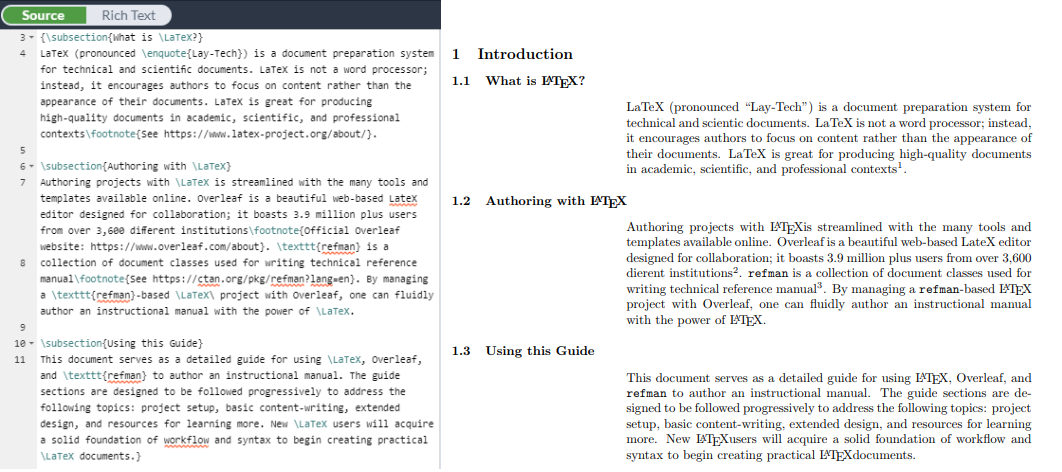
\includegraphics[width=\linewidth]{graphics/IntroSource.png}
\par
\texttt{refman} is a collection of document classes used for writing technical reference manual\footnote{See https://ctan.org/pkg/refman?lang=en}. By managing \texttt{refman}-based projects with Overleaf, authors can fluidly create instructional manuals with the power of \LaTeX.

\subsection{Using this Guide}
This document serves as a detailed guide for using \LaTeX, Overleaf, and \texttt{refman} to author an instructional manual. The guide sections are designed to be followed progressively to address the following topics: project setup, basic content-writing, extended design, and resources for learning more. New \LaTeX\ users will acquire a solid foundation of workflow and syntax to begin creating practical \LaTeX\ documents.}

\section{The Art of Layout-Design}
\label{design}
\label{Layout-Design}
\index{layout design}

\subsection{Common Rules}
\index{rules}

There are almost no common rules because every kind of document has 
different requirements and needs a specific layout. This layout 
should consider \emph{who} will read the document, and \emph{how}.

An important criteria is if the reader will read the document from 
start to end like a detective novel (linear reading) or if he wants to 
find certain information as in a telephone directory or a 
reference manual.  \index{manual}\index{telephone directory}

In addition to that, the layout has to consider certain conventions, 
like the habits of the reader or ``Corporate Design'' \index{corporate 
desing} rules that distinguish publications from different publishers.  
\footnote{Compare the layout of different daily papers or magazines 
like ``page'' or ``invers''.}

\attention
The main purpose of a layout is to make sure the reader finds the 
information he wants and is able to read and understand it easily.
The structure, readability, and consistency of a document is more 
important than it's ``beauty''.\footnote{This is not always true for 
adverts that usually contain no information at all and, picture 
magazines where the beauty of the picture \emph{is} the contents.}

The following ``rules of thumb''\index{rules of thumb} will be valid 
for most applications:

\begin{description}

\item[Line spacing]\index{line spacing}
        The spacing between two lines should be larger than the spacing 
        between two words to guide the eyes of the reader.

\item[Line length]\index{line length}
        The length of a line -- or when using multicolumn layout of a 
        column -- should be about 60 characters. When lines get longer they 
        are more difficult to read and it is easier to go to the wrong line 
        after finishing the current one. Increasing the linespacing may help a 
        little.
        When lines get to short it is difficult to set them justified, and you 
        will get lots of hyphenated words.
        
\item[Page layout]\index{page layout}
        Normal text pages should look the same throughout the document. 
        Figures, tables and special pages like the index need not appear in 
        the same layout but should take as much space as needed.
        
\item[Margin notes]\index{margin notes}
        Margin notes are often more suitable than footnotes because they 
        appear right next to the text they refer to. Special margin notes are 
        the ``attention sign'' or the ``dangerous bend'' that guide the user 
        to important parts of the text.
        
\item[Headings and Footings]\index{headings}\index{footings}
        Headings and footings should make it easier for the reader to orient
        himself in the document. If you expect readers to copy single pages
        from the document they should contain information about the paper as
        a whole, just in case you need more information or want to cite the
        whole paper.
        
        If you expect the document to change often (like software manuals),
        each page should contain a version information or at least a date.
        
\end{description}

\subsection{Special note for technical descriptions}

Let us compare three different layouts and check if they are usable for 
technical descriptions, user's guides and reference manuals.  
\footnote{This hint came from Paul Stiff, who teaches layout design at 
the University of Reading.}

\begin{description}

\item[Plain \TeX]
        The standard format use by plain \TeX\ has the great disadvantage 
        that the lines are much to long, which reduces the readability.
        
\item[Standard-\LaTeX]
        The format used by \LaTeX{}s standard classes isn't ideal. The 
        line length is correct, but that leaves us with a wide unused margin. 
        The font used for section headings is too large. The Koma-Script 
        classes improve this and offer many ways to configure the fonts. 
        This is a good design for a paper one usually reads from start to 
        end.
        
\item[Reference Manual Style]
        A new design that appeared some years ago and is used in recent 
        reference manuals, is much more suited for our purpose.
        \footnote{The ``PostScript Reference Manual'' is one document that 
        uses such a design.}
\begin{itemize}
\item
        The text is printed in rather short lines in the right part of the 
        page. This part is used for continuous reading.
\item
        The wide left margin is used for headings and margin notes. Since 
        you now have a wide margin it is easier to use long margin notes to 
        supply additional information and to lead the reader to important 
        parts of the documents. Please note that the margin is always on the 
        left side thus two-sided printing does not look symmetrical. This is 
        done on purpose, because the reader will always start reading at the 
        left side, and with this layout section headers really ``stand out''. 
        In a symmetrical layout, half the headers would be buried in the text.
\item
        Figures and tables are either inside the text column, inside the
        margin or, if necessary, fill the whole page.
\end{itemize}

\seealso{Section \ref{refmanex}}
Section~\ref{refmanex} describes how to implement such a layout in 
\LaTeX.

\end{description}

%%%%%%%%%%%%%%%%%%%%%%%%%%%%%%%%%%%%%%%%%%%%%%%%%%%%%%%%%%%%%%%%%%%%%%


\section{How to change a \LaTeX\ layout?}
\label{layout}

\subsection{Advantages and Disadvantages of the text processing system \LaTeX}

\marginlabel{Advantages:} The big advantage of \LaTeX\ is, that it 
implements a ``generic'' or ``logical'' design.\index{design, 
logical}\index{design, generic} This means that the author has to 
specify the \emph{meaning} of special parts of the text like: 
headings, citations, lists, literature references, and so on. These 
logical definitions will be processed by the system and printed in 
the ``correct'' way. The meaning of \emph{correct} is defined in the 
document class and additional packages.

The opposite of this is the ``visual'' design\index{design, visual} 
that most text processors use. Here the author has to know the correct 
way to set certain parts of the text and take care of the correct 
printing.

The logical design makes it easier for the author to write 
consistent documents (\ie\ same font and fontsize for section headings 
of the same level, same layout for lists and enumerations, \dots).

\marginlabel{Disadvantages:}
The main disadvantage of \LaTeX\ is that the author has only limited 
means to change the layout and that she has only four classes to 
choose from. This has changed a great deal with the appearance of the 
Script classes for \LaTeX\ 2.09 in 1992, which in turn have been replaced by 
the even more improved Koma-Script classes for \LaTeXe.

Another disadvantage is that \LaTeX\ seems to be tied to the 
``Computer modern'' font family. This is simply not true, at least 
not when you have a PostScript printer. Setting up different fonts 
isn't an easy task, but once they are installed they are as easy 
to use as the standard fonts.

But \LaTeX\ is much more powerful and flexible: you can define an 
arbitrary design by changing the definitions in the class files or 
overwrite them by packages. This is easier than you may think and 
happens more often than you think. Many universities and publishers 
have their own \LaTeX\ class but do not distribute it to the 
world.\footnote{You can find a generic \texttt{elsevier.cls} on CTAN 
which you can use to prepare article before submission. This will be 
replaced by the magazine-specific class at the publisher.}


\subsection{Input files and class files}

According to the principle of separation of content and design, 
there are two kind of files:

\begin{itemize}
\item
        The content and the logical structure of a document are defined in 
        the \LaTeX\ input file.
\item
        The design (layout) is defined in the class files and packages.
\end{itemize}
Which class and packages files a document will use is defined at the 
beginning of the input file.  The \verb|\documentclass| command 
selects the class and the \verb+\usepackage+ command specifies 
additional packages.

To generate a paper you need at least two files, the input file and a 
class file.

These two files represent the work of the author and designer as 
explained in the introduction. Even if the author and the designer are 
the same person, this has some advantages:

\begin{itemize}
\item
        Similar documents (that appear in a series) have the same layout 
        because the layout is defined in a file of its own and not part of 
        the document.
\item
        You can print the same contents without much work in different 
        layouts, \eg\ as an article for a magazine and as a chapter for a 
        dissertation.
\end{itemize}

\subsection{Class files and Packages}

\LaTeX\ supports a hierarchy of layout definitions.
\begin{itemize}
\item
        The first file processed is the class file that is specified inside 
        the curly braces of the \verb|\documentclass| command. This 
        defines the kind of document you want to write. 
\item
        The optional argument of the \verb|\documentclass| command inside 
        the square brackets defines class options which select variants of 
        the basic layout,such as different font sizes.
\item
        The last step is reading the packages specified by the 
        \verb|\usepackage| command. This command again takes options to 
        select the layout.
\item
        You can change layout parameters in the input file, but this is 
        discouraged because it violates the principle of separation of 
        content and design.

\end{itemize}

There are some important differences between class and package files 
and ``normal'' input files:
\begin{itemize}
\item
        Class and package files should only contain definitions. They must 
        not output text.
\item
        The ``at''-sign \texttt{@} is treated as a letter and therefore may 
        appear in command names. Most internal commands of \LaTeX\ contain 
        an \texttt{@} to prevent the author from using them accidentally.
\item
        The extension of the file is \texttt{.cls}, \texttt{.clo} or 
        \texttt{.sty} instead of \texttt{.tex}.
\end{itemize}

\subsection{Changing the layout, step by step}
\index{changing the layout, step by step}

It is usually easier to change existing class files instead of 
writing a new one from scratch. In many cases it is even sufficient 
so replace some definitions and put them into a package instead of 
creating a new class.

Please note that you are \emph{not} allowed to change the standard 
classes distributed with \LaTeX. You \emph{have} to change the name 
when you want to make changes. That is another reason to put small 
changes in packages.

\subsubsection{Defining the differences between the desired  and 
the available layout}

The first step is to define the difference between the layout you have 
and the layout you want. 

\subsubsection{Finding the original definition}

The next step is to find out where the original layout is defined.  It 
is best to search the files in the following order:\footnote{This hint 
came from Sue Brooks, who held a workshop for ``\LaTeX-Hacker'' at the 
1988 \TeX-conference in Exeter.}
\begin{enumerate}
\item the \LaTeX\ manual by Leslie Lamport,
\item the \LaTeX\ documentations files \texttt{*.dtx} for the classes 
or packages
\item the \LaTeX\ documentations files \texttt{*.dtx} for the kernel,
\item the \TeX book by Donald E.~Knuth.
\end{enumerate}

The files are usually documented quite well so you should be able to 
change things even if you don't understand everything.


\subsubsection{Writing a new package file}

The third step is to create a new package. You choose an appropriate 
name for the package (like \texttt{mysty}) and create a filename by 
adding the extension \texttt{.sty}.

This file will only contain the definitions you want to change or the 
new commands you want to define.

If you want to change definitions or certain parameters, the best way 
is to copy them from the original file and modify them according to 
your liking.

Defining new commands is easier when you find similar commands in the 
original files which you can change.

It is always a good idea to include the reason you wrote the package, 
the changes it makes and the new commands it defines in the file. You 
should include the date of the last change and the \LaTeX\ version it 
works with, just in case some internal \LaTeX\ commands you use will change.

When writing larger packages, it is an even better idea to use the 
\texttt{docstrip} program which is used to document the \LaTeXe\ files.  Thus 
you have your code and documentation in one file and it's easier to 
keep them from going out of sync.

\subsubsection{Using the new package}

To use the new package, you call it with the \verb|\usepackage| command. 
This command executes the code of your package and changes the layout 
as desired.

Example:

\begin{verbatim}
   \documentclass[11pt,twoside,a4paper]{article}
   \usepackage{mysty} %<- This calls the package "mysty"
\end{verbatim}

You shouldn't need to change anything else in your input file, unless 
you defined new commands or environments that are not available in 
standard \LaTeX.

\attention
When you copy your input file to a different computer you have to 
include your new packages as well. Otherwise the document can't be 
processed.

%%%%%%     %%%%%%%%%%      %%%%%%%%%%        %%%%%%%%%%        %%%%%%%%%

\subsection{A simple example (Equation numbers)}

Let's assume that you want to write an article where the equations are 
numbered separately in every section. In the \LaTeX\ manual you find a 
notice that the report class does something similar for every chapter.

Looking into the file \texttt{report.cls} you will find the following 
commands that deal with equation numbers:\nopagebreak
\begin{verbatim}
   \@addtoreset{equation}{chapter}
   \def\theequation{\thechapter .\arabic{equation}}
   % or in LaTeX2e since 1995/06/01:
   \renewcommand\theequation{
                \thechapter.\@arabic\c@equation
                                }
\end{verbatim}

You don't necessarily need to understand these two commands in detail.

Now you create an new file with the name 
\texttt{eqpersec.sty}\footnote{Depending on the computer you are using 
the name may be different like \texttt{EQPERSEC\_STY} on a CYBER 
running NOS/VE. But note that you must not use spaces in the 
filename.} and copy the commands above into that file.  After that 
you replace every occurrence of \texttt{chapter} with \texttt{section} 
and add some comments.\nopagebreak
\begin{verbatim}
   % This is equation_per_section.sty
   % Short name: eqpersec.sty
   % Original file by Hubert Partl 1988
   % Modified by Axel Kielhorn 1996/01/01
   % to support LaTeX 1995/06/01 and later
   %
   % reset the equation counter at the start
   % of a new section 
   % 
   \@addtoreset{equation}{section}
   % Equationnumber = sectionnummer.equationnummer
   % Use only one of the below 
   % depending on you LaTeX version
   % 
   %\def\theequation{\thesection .\arabic{equation}}
   % or in more recent versions of LaTeX
   \renewcommand\theequation{
                \thesection.\@arabic\c@equation
                                }
\end{verbatim}


Whenever you use a \verb|\usepacakge{eqpersec}| command as in
\nopagebreak
\begin{verbatim}
\documentclass[11pt]{article}
\usepackage{eqpersec}
\end{verbatim}
you will get equations numbered according to your conventions.


%%%%%%%%%% %%%%%%%%%%%%%% %%%%%%%%%%%% %%%%%%%%%%%% %%%%%%%% %%%%%%%%%%%%

\subsection{A more complex example (Reference Manual)}
\label{refmanex}

We want to create a layout similar to the one used in the \textit{PostScript 
Reference Manual}, with a wide left margin for headings and margin 
notes and a small margin at the right and bottom.

\subsubsection{Page layout}

To define the new layout we use the commands described in the \LaTeX\ 
manual. For full details see the file \texttt{refman.dtx}.

%\pagebreak[2]

\marginlabel{Horizontal:}
First we define two new names for length that we will use often:

\cs{fullwidth} is the width of the whole page minus a margin of 1~inch 
on every side. 
%
\begin{displaymath}
\texttt{fullwidth} = \texttt{paperwidth} - 2\ \textrm{inch}
\end{displaymath}
%
From this the width of the text is calculated.
%
\begin{displaymath}
\texttt{textwidth} = \texttt{fullwidth} \times \texttt{textfraction}
\end{displaymath}
%
\cs{leftmarginwidth} is the width of the left margin that will be 
used for headings and margin notes. 
\begin{displaymath}
\texttt{leftmarginwidth} = \texttt{fullwidth} - \texttt{textwidth}
\end{displaymath}
%
This is a little more difficult in reality because the lengths have to 
be rounded to full points and a possible two column layout -- as used 
in the index -- must be taken into consideration.

\marginlabel{Vertical:}
The vertical layout is a little more difficult because you have to 
deal with the page header and footer. 
%
\begin{displaymath}
\texttt{textheight} = \texttt{paperheight} - 2.5\ \textrm{inch}
\end{displaymath}
%
The result of this calculation is rounded to full lines. Depending on 
the page style -- headings or footings -- it is shifted up or down by one 
line.

\vspace{0pt plus 1cm}

\subsubsection{Section headings}

The headings have to be modified to make them extend into the left 
margin.

In file \texttt{classes.dtx} we find the \verb|\@startsection| command 
that defines the layout of the headings. Only parameters 4 to 6 are 
relevant for us: parameter 4 is the space above and parameter 5 the 
space below the section. The 6th parameter does the actual formatting.

This is the original definition:\nopagebreak
\begin{verbatim}
\newcommand\section{\@startsection
             {section}{1}{\z@}%
             {-3.5ex plus -1ex minus -.2ex}%
             {2.3ex plus .2ex}%
             {\normalfont\Large\bfseries}}
\end{verbatim}

The commands for sub- and subsubsections are similar. Note that the 
measures are all in \texttt{ex}, thus depending on the font size used.

We define a new command \cs{secshape} to format the headings. This 
command uses the whole width of the page for the heading. To discourage 
hyphenation of the heading we give it a high penalty. This still 
allows hyphenation when absolutely necessary.

\begin{verbatim}
\newcommand\secshape{%
               \leftskip=-\leftmarginwidth%
               \rightskip=\@flushglue%
               \hyphenpenalty=2000}
\end{verbatim}

This command is inserted into the 6th parameter of \verb|\@startsection|.

Since the headings now extend into the left margin, we can use a 
smaller font and reduce the space between the text and the heading. The 
new definition looks like the following:\nopagebreak
\begin{verbatim}
\newcommand\section{\@startsection
             {section}{1}{\z@}%
             {-2ex plus -1ex minus -.2ex}%
             {0.5ex plus .2ex}%
             {\secshape\normalfont\large\bfseries}}
\end{verbatim}

\vspace{0pt plus 1cm}

\subsubsection{Setting the margin notes}

The margin notes should always appear on the left side of the text. 
The normal layout puts them into the outer margin in twoside layout.

The file \texttt{latex.dtx} contains the definition of the 
\verb|\@addmarginpar| command which is responsible for the margin 
notes. We don't have to understand the whole definition; the important 
part is the internal variable \verb|\@tempcnta| that is either 
\verb|\@ne| (1) when the note should appear on the right side of the 
text or \verb|\m@ne| ($-1$) when it should appear on the left side.

This is done by the following lines:
\begin{verbatim}
    \@tempcnta\@ne
    \if@twocolumn
        \if@firstcolumn \@tempcnta\m@ne \fi
    \else
      \if@mparswitch
         \ifodd\c@page \else\@tempcnta\m@ne \fi
      \fi
      \if@reversemargin \@tempcnta -\@tempcnta \fi
    \fi
\end{verbatim}

which we simply replace by:
\begin{verbatim}
    \@tempcnta\m@ne
\end{verbatim}

The remaining lines that handle the setting of the margin note 
depending on the parameter \verb|\@tempcnta| are left unchanged.

\subsubsection{Extensions}

The definitions described above are sufficient for simple applications 
but in practical use one may want some additional commands.  
\seealso{Appendix \ref{refman}} You will find the description for the whole new 
class in the appendix~\ref{refman}.

%%%%%%%%%%%%%%%%%%%%%%%%%%%%%%%%%%%%%%%%%%%%%%%%%%%%%%%%%%%%%%%%%%%%%%

\input lay_e2

%%%%%%%%%%%%%%%%%%%%%%%%%%%%%%%%%%%%%%%%%%%%%%%%%%%%%%%%%%%%%%%%%%%%%%

\printindex

\end{document}
